% ******************************************************** %
%              TEMPLATE DE INFORME ORGA2 v0.1              %
% ******************************************************** %
% ******************************************************** %
%                                                          %
% ALGUNOS PAQUETES REQUERIDOS (EN UBUNTU):                 %
% ========================================
%                                                          %
% texlive-latex-base                                       %
% texlive-latex-recommended                                %
% texlive-fonts-recommended                                %
% texlive-latex-extra?                                     %
% texlive-lang-spanish (en ubuntu 13.10)                   %
% ******************************************************** %


\documentclass[a4paper]{article}
\usepackage[spanish]{babel}
\usepackage[utf8]{inputenc}
\usepackage{charter}   % tipografia
\usepackage{graphicx}
%\usepackage{makeidx}
\usepackage{paralist} %itemize inline

%\usepackage{float}
%\usepackage{amsmath, amsthm, amssymb}
%\usepackage{amsfonts}
%\usepackage{sectsty}
%\usepackage{charter}
%\usepackage{wrapfig}
\usepackage{listings}
\lstset{language=C}
\usepackage{caption}
\usepackage{color}

% \setcounter{secnumdepth}{2}
\usepackage{underscore}
\usepackage{caratula}
\usepackage{url}
\usepackage[document]{ragged2e}
\usepackage[export]{adjustbox}
\usepackage{subcaption}
\usepackage{floatrow}


% ********************************************************* %
% ~~~~~~~~              Code snippets             ~~~~~~~~~ %
% ********************************************************* %

\usepackage{color} % para snipets de codigo coloreados
\usepackage{fancybox}  % para el sbox de los snipets de codigo

\definecolor{litegrey}{gray}{0.94}

\newenvironment{codesnippet}{%
	\begin{Sbox}\begin{minipage}{\textwidth}\sffamily\small}%
	{\end{minipage}\end{Sbox}%
		\begin{center}%
		\vspace{-0.4cm}\colorbox{litegrey}{\TheSbox}\end{center}\vspace{0.3cm}}



% ********************************************************* %
% ~~~~~~~~         Formato de las páginas         ~~~~~~~~~ %
% ********************************************************* %

\usepackage{fancyhdr}
\usepackage{parskip}
\pagestyle{fancy}

%\renewcommand{\chaptermark}[1]{\markboth{#1}{}}
\renewcommand{\sectionmark}[1]{\markright{\thesection\ - #1}}

\fancyhf{}

\fancyhead[LO]{Sección \rightmark} % \thesection\
\fancyfoot[LO]{\small{Kevin Frachtenberg,Nicolas Bukovits}}
\fancyfoot[RO]{\thepage}
\renewcommand{\headrulewidth}{0.5pt}
\renewcommand{\footrulewidth}{0.5pt}
\setlength{\hoffset}{-0.8in}
\setlength{\textwidth}{16cm}
%\setlength{\hoffset}{-1.1cm}
%\setlength{\textwidth}{16cm}
\setlength{\headsep}{0.5cm}
\setlength{\textheight}{25cm}
\setlength{\voffset}{-0.7in}
\setlength{\headwidth}{\textwidth}
\setlength{\headheight}{13.1pt}
\setlength{\parindent}{4em}
\setlength{\parskip}{\baselineskip}

\renewcommand{\baselinestretch}{1.1}  % line spacing

% ******************************************************** %


\begin{document}


\thispagestyle{empty}
\materia{Sistemas Operativos}
\submateria{Primer Cuatrimestre de 2018}
\titulo{Trabajo Práctico 1}
\subtitulo{Pthreads}
\integrante{Kevin Frachtenberg}{247/14}{kevinfra94@gmail.com}
\integrante{Nicolas Bukovits}{546/14}{nicko_buk@hotmail.com}
\maketitle

%{\small\textbf{\flushleft{Resumen}}\\
\abstract {En el siguiente trabajo pr\'actico, se realiz\'o una implementaci\'on de un ConcurrentHashMap el cual es una tabla de hash abierta, que significa que en caso de colisión se genera una lista enlazada dentro del bucket. Esta lista tiene la particularidad de poder ser utilizada por threads concurrentes. Su interfaz de uso es como un diccionario. Las claves son strings y los valores son enteros.

%\newpage

%\thispagestyle{empty}
%\vfill


\thispagestyle{empty}
\vspace{3cm}
\tableofcontents
\newpage


%\normalsize
\newpage



\section{Resolucion de Ejercicios}
\subsection{Ejercicio 1}

En este ejercicio se completó la implementación del método push_front de la lista atómica provista por la cátedra. El método fue crear un nuevo nodo. Al nuevo nodo se le cargó como nodo siguiente el nodo inicial actualmente. Se compara atomicamente el valor del actual nodo inicial con el siguiente del nuevo nodo inicial. Si son iguales reemplaza el valor del actual nodo incial con el nuevo nodo creado. Si no son iguales se vuelve a recuperar el nodo inicial y se intenta nuevamente. \newline
Luego se procedió a implementar la clase ConcurrentHashMap, la cual contiene un constructor que crea una tabla con 26 entradas (una por cada letra del abecedario) en la cual en cada una hay una lista de pares {\tt $<$string, entero$>$ } para que la tabla sea de hashing abierto y en caso de colisión se agregue la nueva palabra al principio de la lista. La función de Hash es simplemente tomar la primera letra de la palabra, por lo que para cada existe una entrada en la tabla. Además de crearse e inicializarse la tabla, se crea un array de 26 mutex llamando a la función {\tt pthread_mutex_init } para que durante el uso de threads, podamos asegurarnos que solo uno escribe la tabla al mismo tiempo. \newline
% revisar este itemize. para mi habria que hacerlo mas "prosa" como hice arriba. si no, volaro lo de arriba.
Luego de haber completado la implementación de la lista se debe implementar la clase ConcurrentHashMap con las siguientes especificaciones: 

\begin{itemize}

\item ConcurrentHashMap(): Constructor .Crea la tabla. La misma tendrá 26 entradas (una por
cada letra del abecedario). Cada entrada consta de una lista de pares (string, entero). La
función de hash será la primer letra del string. Para ello se crea una nueva lista en cada una de las entradas y se inicializan los mutex de cada entrada de la tabla llamando a la función pthread_mutex_init.\blindtext
\item void addAndInc(string key): Si key existe, incrementa su valor, si no existe, crea el par
(key, 1). Se debe garantizar que sólo haya contención en caso de colisión de hash. Esto es,
deberá haber locking a nivel de cada elemento del array. Para implementarlo primero se obtiene la posición en la tabla usando la función de hash. Se pide el mutex de la entrada correspondiente y si la clave no esta definida se agrega al principio de la lista el par (key,0). Se realiza un unlock de la entrada y se recorre toda la lista de la posición en la tabla usando el iterador. Cuando se encuentra a la clave se pide el mutex y se incrementa en uno el valor entero del par (clave,valor). Luego se vuelve a desloquear la entrada.\blindtext
\item bool member(string key): true si y solo si el par (key, x) pertenece al hash map para algún
x. Esta operación deberá ser wait-free. Simplemente esta función recupera la posición en la tabla y con el iterador recorre la lista. Si encuentra la clave definida devuelve verdadero. 
\item {\tt pair<string, unsigned int>maximum(unsigned int nt) }: devuelve el par (k, m) tal que
k es la clave con máxima cantidad de apariciones y m es ese valor. No puede ser concurrente
con addAndInc, si con member, y tiene que ser implementada con concurrencia interna. El
parámetro nt indica la cantidad de threads a utilizar. Los threads procesarán una fila del
array. Si no tienen filas por procesar terminarán su ejecución. La implementación consistió en definir un entero atómico y un Elem atómico que se van a usar para llevar registro de la cantidad de posiciones de la tabla a analizar y el elemento máximo encontrado. Se crean los nt threads, se pide el mutex de todas las entradas de la tabla, se cargan todas las estructuras auxiliares que van a usar los threads y se lanzan a correr los threads a los cuales se le pasa como paŕametro una función max_thread. La misma incrementa en uno atómicamente a la variable siguiente y mientras siguiente sea menos que 26, se recorre la lista en cada posicion y se va actualizando atomicamente el valor del Elem atómico que representa el máximo. Se espera a que todos los threads terminen y se hace un unlock de todas las entradas de la tabla.

\end{itemize}

\subsection{Ejercicio 2}

En este ejercicio se implementó una función ConcurrentHashMap count_words(string arch) que toma un archivo de texto y devuelve un ConcurrentHashMap cargado con las palabras del archivo. Las palabras se consideran separadas por espacio. Debe ser no concurrente.
Para realizar lo pedido la función abre el archivo y llama a la función getline que toma el arhivo, un string y un caracter delimitador. Mientras haya palabras para leer se van cargando en el string y por cada una de ellas se agregan al ConcurrentHashMap usando la función addAndInc implementada en el ejercicio anterior. Una vez que se hayan leido todas las palabras se cierra el archivo.


\subsection{Ejercicio 3}

En este ejercicio se implementó una función {\tt count_words(list<string>archs)} que toma como parámetros una lista de archivos de texto y devuelve un ConcurrentHashMap cargado con las palabras. Utiliza un thread por archivo.
Para ello se crean tantos pthread_t como archivos se reciben por parametro. Se crean n {\tt pair$<$string*,ConcurrentHashMap*$>$} siendo n la cantidad de archivos. Se itera por cada archivo y se carga un {\tt pair$<$string*,ConcurrentHashMap*$>$} para cada thread. En el mismo se carga el archivo y la referencia de un ConcurrentHashMap. Se llama a la función {\tt pthread_create} al cual se le pasa el pthread_t creado, la función que va a ser la que va a ejecutar el thread que es count_words_threads y la referencia al par creado. La función {\tt count_words_threads} recibe el input del {\tt pair$<$string*,ConcurrentHashMap*$>$} y llama a la función {\tt count_words} con el nombre del archivo. Se espera a que todos los threads terminen llamando n veces a la función {\tt pthread_join}. Se devuelve el ConcurrentHashMap que cargaron los threads.


\subsection{Ejercicio 4}
En este ejercicio se implementó una función {\tt count_words(unsigned int n, list<string>archs)} que hace lo mismo que la anterior función pero utiliza n threads, pudiendo ser n menor que la cantidad de archivos. Similar a la función anterior pero crea n threads. Se le pasa a cada thread una estructura que contiene el nombre de los archivos y mientras no se hayan cargado todos los archivos los threads llaman a la función {\tt count_words(file,ConcurrentHashMap)}.

\subsection{Ejercicio 5}
En este ejercicio se implementó una función {\tt maximum(unsigned int p_archivos, unsigned int p_maximos, list<string>archs)} que retorna un par con un string como primer elemento que representa la palabra que mas apariciones tiene y un entero como segundo elemento que es la cantidad de apariciones. Utiliza p_threads threads para leer los archivos y p_maximos threads para calcular los máximos. No se utilizó las versiones concurrentes de la función count_words. Similar al maximum pero crea p_archivos threads para leer los archivos que funciona como el ejercicio anterior y utiliza p_maximos threads que llenan un ConcurrentHashMap general al que despúes se le calcula el maximo usando la función maximum.


\subsection{Ejercicio 6}

En este ejercicio se implementó la misma funcionalidad del ejercicio anterior pero utilizando la versión concurrente de count_words del ejercicio 4. La segunda parte de la funcion, realiza el mismo procedimiento que la funcion maximum del ejercicio 5.

Para comparar resultados, creamos un archivo max-compare que sirve para ejecutar una vez cada función {\tt maximum } con {\tt p_archivos } y {\tt p_maximos } pasados por parametro. Luego creamos un script en shell para ejecutar max-compare 500 veces tomando la cantidad maxima de {\tt p_archivos } por parametro y fijando el parametro {\tt p_maximos } en 5, ya que justamente la segunda parte de las funciones {\tt maximum } se mantuvieron similares. Los resultados de la corrida del script con hasta 5 threads fueron los siguientes:

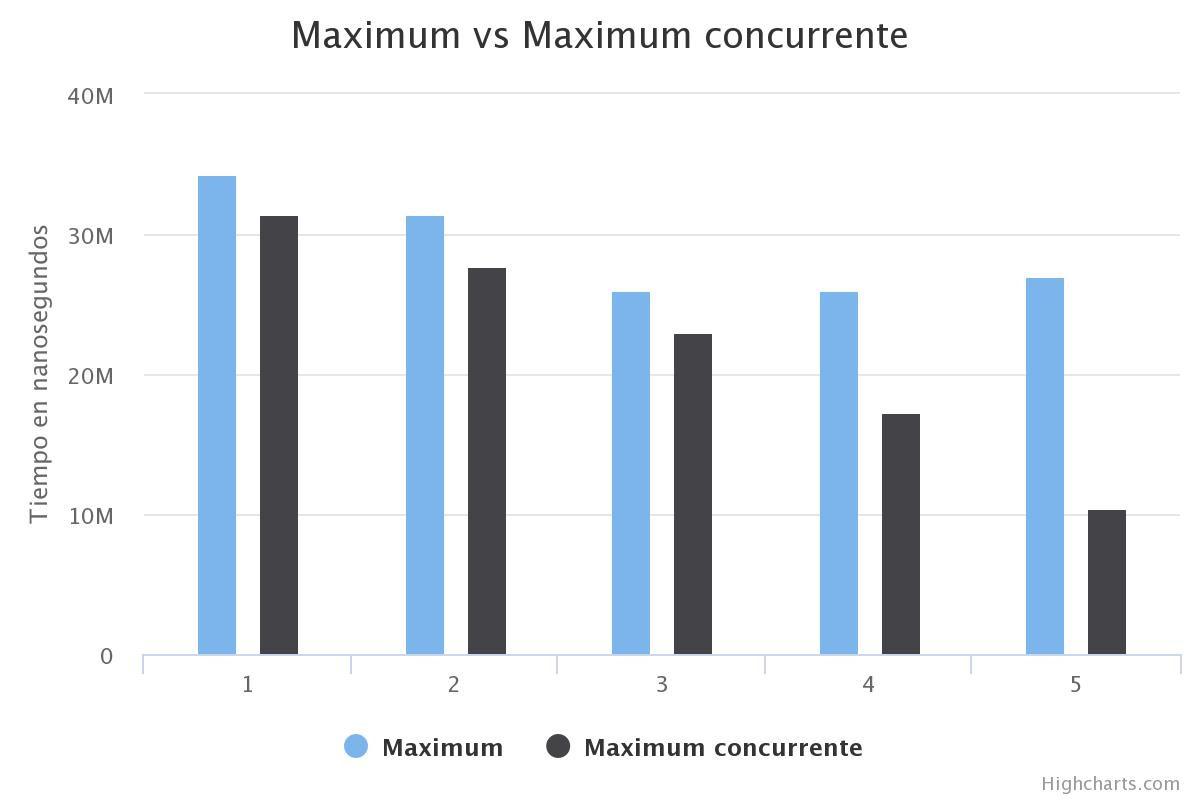
\includegraphics[scale=0.35]{imagenes/chart.jpeg}

Se esperaba que la funcion maximum_concurrent ejecute mas rápido que la función maximum. Sin embargo luego de ver los resultados de la exerimentación y analizar el código se llegó a la conclusión de que la función maximum es más rápida ya que hace un mejor uso de los threads. Se observó que a mayor cantidad de threads los tiempos de ejecución diminuían para ambas funciones.


\section{Detalles implementativos y pruebas}
Para seguir las consignas del enunciado en las cuales se pedia que solamente las funciones del primer ejercicio pertenezcan a la clase ConcurrentHashMap, fue necesario modificar los tests provistos por la catedra, ya que asumian que funciones como el count_words estaban en el namespace de la clase ConcurrentHashMap, cuando en realidad no.
\newline
Se agregó el archivo test-1.cpp el cual incluye tests particulares sobre ConcurrentHashMap. El archivo tiene tres partes en el cual se prueban las funciones member,addAndInc y maximum del ConcurrentHashMap, las cuales para poder ejecutarse prueban también el constructor del mismo. Para poder realizar los tests fue necesario agregar funciones auxiliares que se usan para este fin las cuales son add, Inc y count_word. Estas funciones fueron agregadas para testear member,addAndInc y maximum sin asumir que las demas funcionan excepto el maximum. Los tests se desarrollaron de manera incremental empezando con member, luego una vez que se testeo correctamente member, se testeó addAndInc y finalmente maximum.


\end{document}
